% 96-45(96쪽) — 삼각형 ABC 의 세 변을 $2:1$ 로 내분하는 점 P·Q·R 와 삼각형 PQR(원문 「오른쪽 그림」). 스캔 화질이 낮아 TikZ 로 다시 그림.
% 라벨은 원문 것만: 꼭짓점 A·B·C 와 내분점 P·Q·R. 넓이의 비(답)가 읽히지 않게 길이·눈금은 적지 않는다.
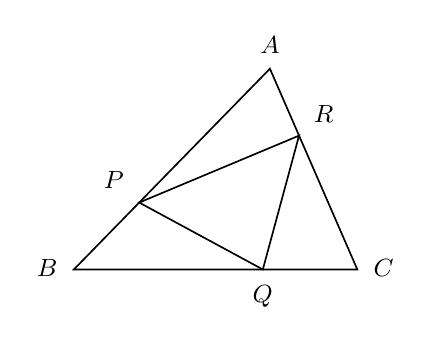
\begin{tikzpicture}[line width=0.6pt, x=1cm, y=1cm]
  \coordinate (B) at (0,0);
  \coordinate (C) at (3.6,0);
  \coordinate (A) at (2.49,2.55);
  \coordinate (P) at (0.83,0.85);
  \coordinate (Q) at (2.40,0);
  \coordinate (R) at (2.86,1.70);
  \draw (A) -- (B) -- (C) -- cycle;
  \draw (P) -- (Q) -- (R) -- cycle;
  \node[font=\small, anchor=south] at (2.49,2.61) {$\pt{A}$};
  \node[font=\small, anchor=east] at (-0.08,0.02) {$\pt{B}$};
  \node[font=\small, anchor=west] at (3.68,0.02) {$\pt{C}$};
  \node[font=\small, anchor=south east] at (0.76,0.90) {$\pt{P}$};
  \node[font=\small, anchor=north] at (2.40,-0.08) {$\pt{Q}$};
  \node[font=\small, anchor=south west] at (2.92,1.74) {$\pt{R}$};
\end{tikzpicture}
